\documentclass{beamer}
\usepackage{lmodern}
\usetheme{Madrid}
\usepackage{multirow}
\setbeamertemplate{background}{\tikz[overlay,remember picture]\node[opacity=0.25]at (current page.center){
\includegraphics[width=14cm]{Kcolor}};}
\usepackage{tikz}
\usepackage{kantlipsum}

% Change base colour beamer@blendedblue (originally RGB: 0.2,0.2,0.7)
\colorlet{beamer@blendedblue}{blue!46!green}
\usepackage[english]{babel}
\usepackage{apacite}
\usepackage{marvosym}
\usepackage{subfig}
\usepackage{graphicx}
\usepackage[utf8x]{inputenc}
\usepackage{url}
\usepackage{hyperref}
\usepackage{times}
\usepackage{pxfonts}
\usepackage{fontenc}
%\usepackage[dvipsnames]{xcolor}
\setbeamertemplate{bibliography item}[text]
\setbeamercolor{titlelike}{parent=structure}
\setbeamercolor*{title}{fg=blue!46!green}
\title[Investigación con n $\geq$ 10K]{¿Muestras n$\geq$10K en Consumidor?}


\author[Juan C. Correa; Twitter: @jcorrean]{Juan C. Correa Ph.D.} 

\institute[]
{
  Konrad Lorenz Fundación Universitaria\\
  Grupo de Investigación en Psicología del Consumidor\\
  Facultad de Psicología\\
  Bogotá, Colombia\\
  \color{blue}\Email  
\texttt{\href{mailto:juanc.correan@konradlorenz.edu.co}{juanc.correan@konradlorenz.edu.co}}}


\pgfdeclareimage[height=0.6cm]{Klogo}{Klogo}
 \logo{\pgfuseimage{Klogo}}
\setbeamertemplate{caption}[numbered]
\date[Bogotá, Julio, 2020] % (optional)
{\textcolor{blue!46!green}{Ciclo de Charlas Prácticas de Consumo Digital}}

\subject{}
\begin{document}
\begin{frame}
  \titlepage
\end{frame}

\setbeamertemplate{background}{\tikz[overlay,remember picture]\node[opacity=0.2]at (current page.center){
\includegraphics[width=14cm]{Kcolor}};}

\begin{frame}
\frametitle{Agenda} 
\tableofcontents
\end{frame}

% Section and subsections will appear in the presentation overview
% and table of contents.

\setbeamertemplate{background}{\tikz[overlay,remember picture]\node[opacity=0.1]at (current page.center){\includegraphics[width=14cm]{}};}

%\section{Nuestro Equipo}
%\begin{frame}{Nuestro Equipo}
% \begin{figure}
%        \centering
%        \includegraphics[width=1\textwidth]{nosotros}
%    \end{figure}
%\end{frame}

\setbeamertemplate{background}{\tikz[overlay,remember picture]\node[opacity=0.2]at (current page.center){
\includegraphics[width=14cm]{Kcolor}};}

\section{Motivación}
\begin{frame}{Motivación}
\begin{figure}
\centering
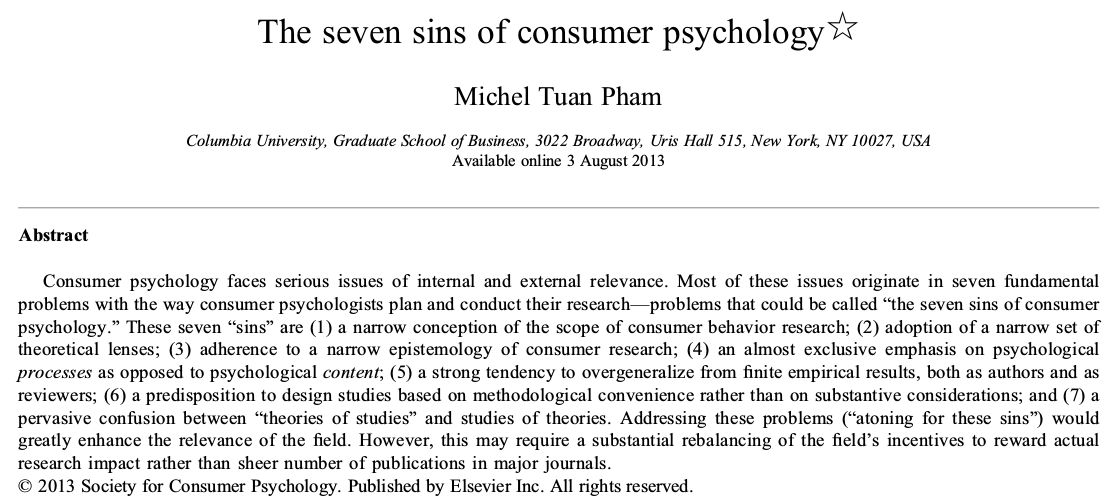
\includegraphics[width=0.9\textwidth]{Pham.png}
\end{figure}    
\end{frame}

\begin{frame}{Motivación}
\textit{``Nosotros deberíamos estar dispuestos a  \textbf{aumentar nuestros tamaños de muestra} para reducir el chance de resultados falso-positivos. Además, necesitamos ser más cuidadosos y ponderados al escribir y discutir los resultados empíricos. Finalmente, necesitamos mayor transparencia sobre los detalles de metodología para aumentar la interpretabilidad y replicabilidad de nuestros hallazgos.''}
\cite[p. 419]{Pham2013}
\end{frame}


\begin{frame}{Motivación}
\Large
\centering
¿Cuán frecuente son los grandes tamaños muestrales en las investigaciones de psicología del consumidor?
\end{frame}


\section{Casos de Estudio}
\begin{frame}
    \centering
    \Huge
    \textit{Dos publicaciones KL\\
    versus \\
    publicaciones en Journal of Consumer Psychology}
\end{frame}

\subsection{Caso 1: Consumo Colaborativo}
\begin{frame}{Caso 1: Consumo Colaborativo}
\begin{figure}
\centering
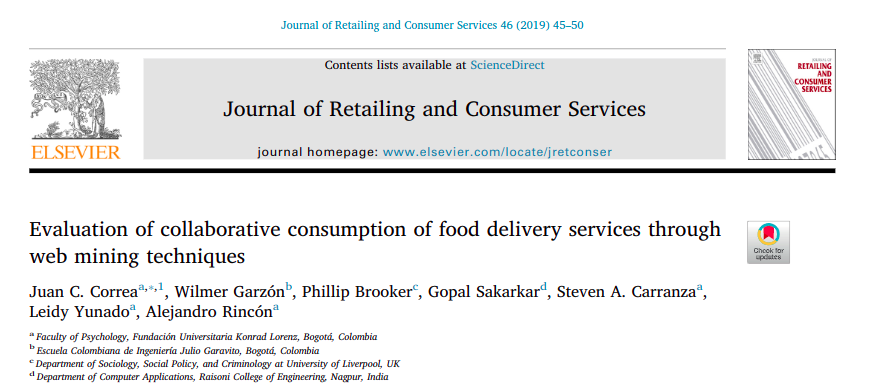
\includegraphics[width=1\textwidth]{Paper2.png}
\end{figure}
\end{frame}

\begin{frame}{Caso 1: Consumo Colaborativo}
El consumo colaborativo ocurre cuando se intercambian bienes o servicios sin la necesidad de usar el dinero; por ejemplo, donaciones, trueques, o comentarios sobre un la calidad de un producto o servicio \cite{Correa2019}. 
\end{frame}

\begin{frame}{Caso 1: Consumo Colaborativo}
\begin{figure}
\centering
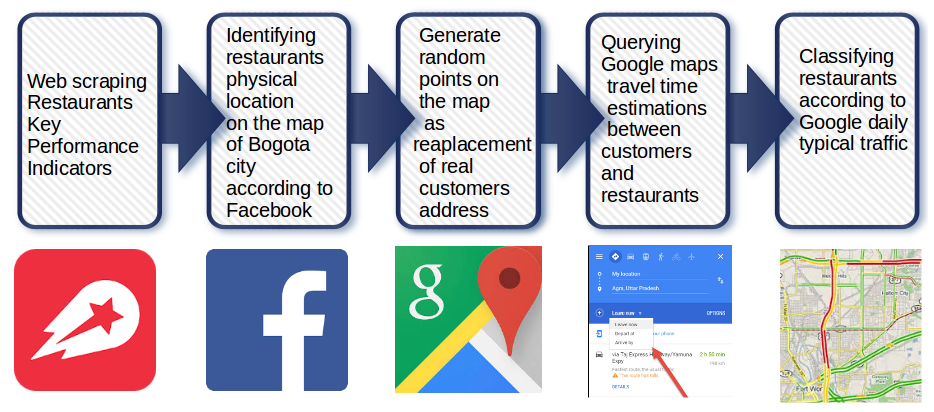
\includegraphics[width=0.9\textwidth]{procedure.png}
\end{figure}
Muestra = 19.934 rutas, 787 restaurantes, 4296 clientes, 3 perídos de observación en las horas pico de los sábados \cite{Correa2019}
\end{frame}

\begin{frame}{Caso 1: Consumo Colaborativo}
\begin{figure}
\centering
 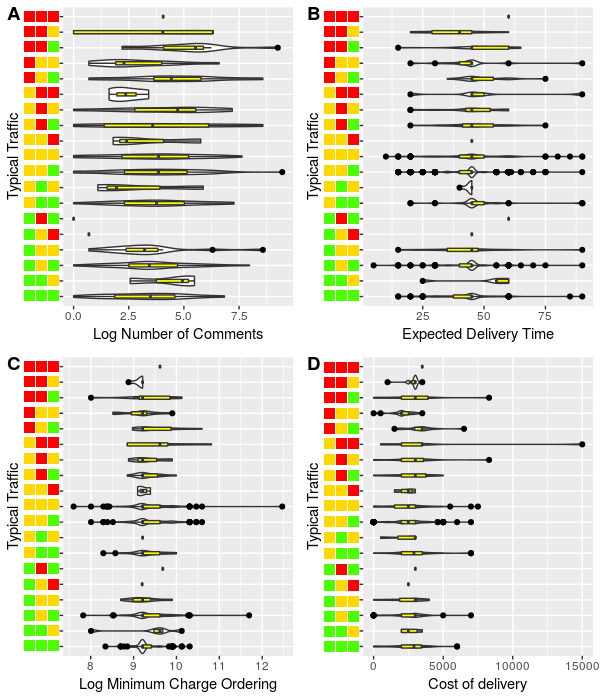
\includegraphics[width=.45\textwidth]{Fig1}
\end{figure}
\end{frame}

\begin{frame}{Caso 1: Consumo Colaborativo}
\begin{figure}
\centering
 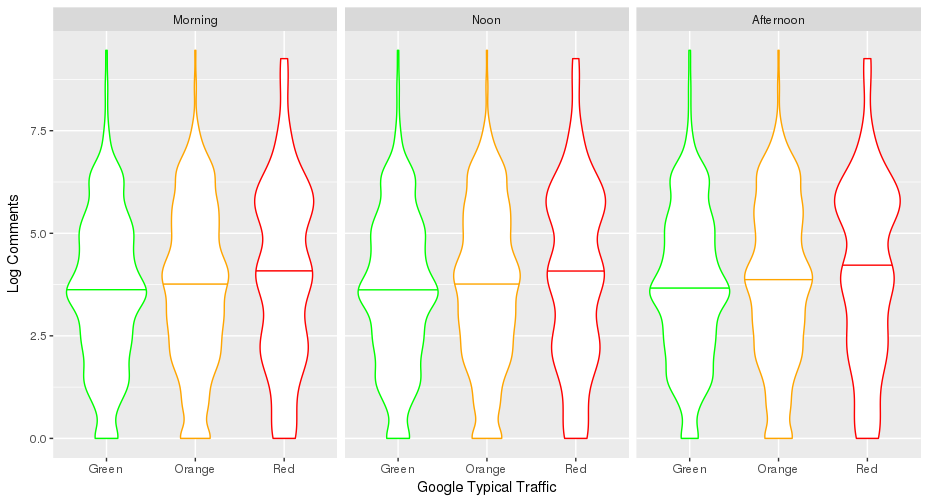
\includegraphics[width=.85\textwidth]{Fig2}
\end{figure}
\end{frame}

\begin{frame}{Caso 1: Consumo Colaborativo}
\begin{figure}
\centering
 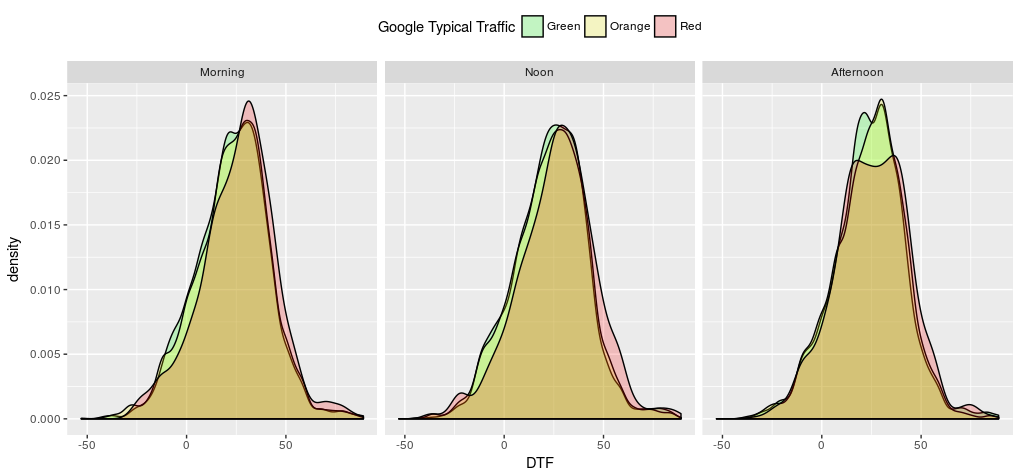
\includegraphics[width=.95\textwidth]{Fig3}
\end{figure}
\end{frame}

\begin{frame}{Caso 1: Consumo Colaborativo}
\begin{figure}
\centering
 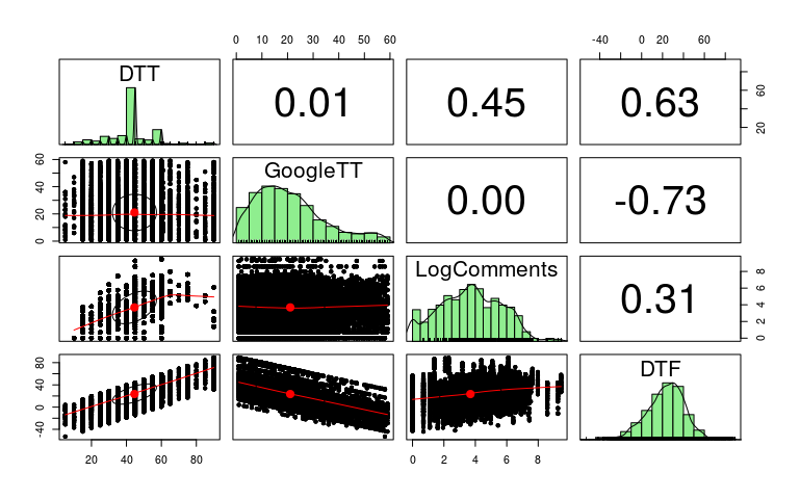
\includegraphics[width=.79\textwidth]{Fig4}
\end{figure}
\end{frame}

\begin{frame}{Caso 1: Consumo Colaborativo}
\begin{itemize}
    \item[1] Los domicilios en Bogotá, en promedio, tardan el tiempo que prometen los restaurantes.
    \pause
    \item[2] Pero los tiempos prometidos para entregar los domicilios no tienen nada que ver con las contingencias en tiempo real del tráfico.
    \pause
    \item[3] La correlación entre tiempos de entrega y el número de comentarios is más bien baja. 
    \pause
    \item[4] El estudio mostró una aproximación novedosa para estudiar la relación entre consumo y mobilidad urbana.
\end{itemize}
\end{frame}

\subsection{Caso 2: Consumo Ideológico}
\begin{frame}{Caso 2: Consumo Ideológico}
El consumo ideológico ocurre cuando la decisión de compra de algún producto o servicio está influenciada por convicciones personales, éticas, políticas o de otra naturaleza \cite{Correa2017}.
\begin{figure}
\centering
 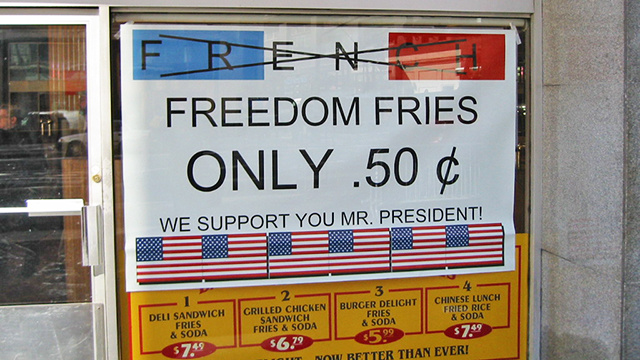
\includegraphics[width=.6\textwidth]{freedomfries.jpeg}
\end{figure}    
\end{frame}


\begin{frame}{Caso 2: Consumo Ideológico}
\begin{figure}
\centering
 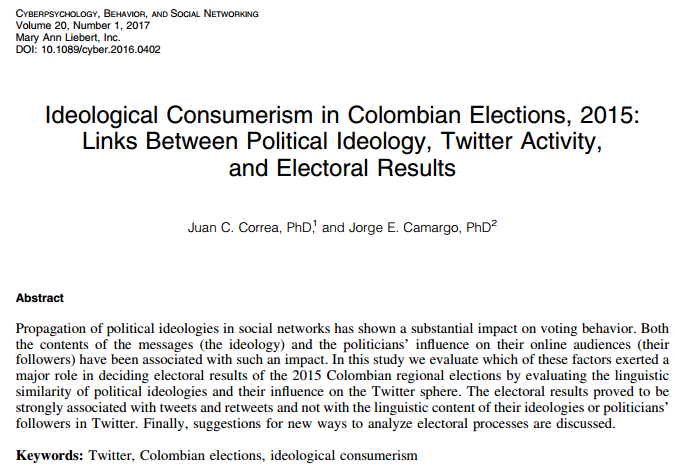
\includegraphics[width=.75\textwidth]{paper}
\end{figure}    
Con 3 sesiones de 5 minutos cada semana de Octubre 2015, se recogieron 69,202 tweets  \cite{Correa2017}
\end{frame}

\begin{frame}{Caso 2: Consumo Ideológico}
\begin{figure}
\centering
 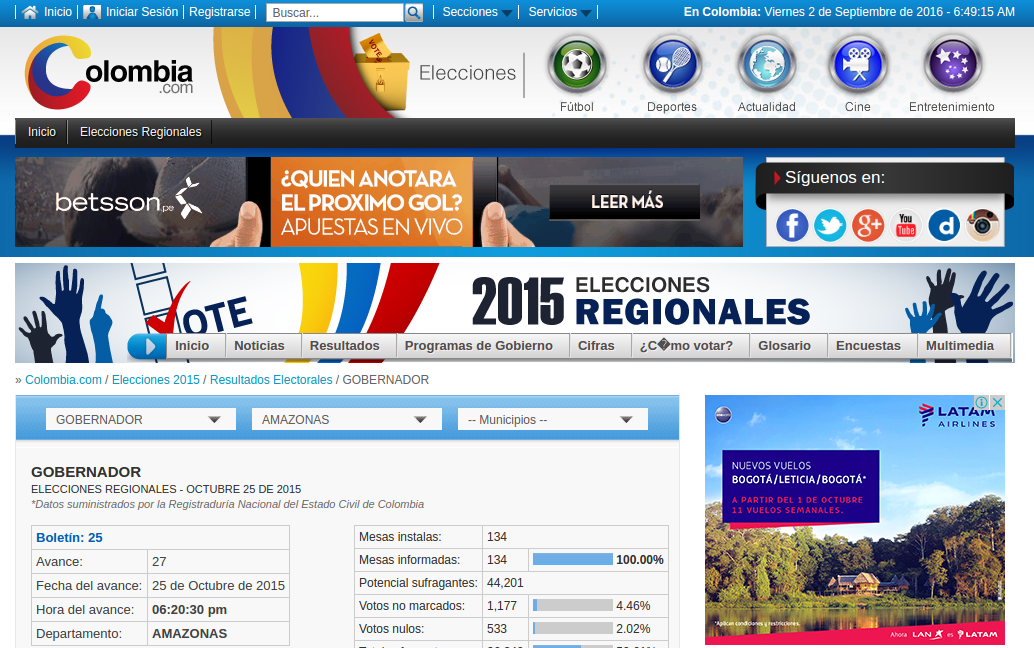
\includegraphics[width=.5\textwidth]{art3.png}
\end{figure}
Usamos una técnica llamada web scraping \cite{Munzert2014} para recolectar datos oficiales de las elecciones, y la API de Twitter API para recoger los tweets de los candidatos a gobernaciones.
\end{frame}

\begin{frame}{Caso 2: Consumo Ideológico}
¿Se puede cuantificar las diferentes ideologías políticas expresadas por los candidatos a gobernaciones en Colombia? 
\begin{equation}
    x_i = (x_{1,i}, x_{2,i}, ..., x_{t, i})
\end{equation}

\begin{equation}
    x_{t, i} = tft \times log|D| / |t \in i|
\end{equation}
Aquí $tft$ representa la frecuencia de palabras $t$ en un tweet.
$i$, $|D|$ es el número de tweets que componen una colección de tweets, y $log|D| / |t \in i|$ es el inverso de la frecuencia de esos tweets $t$ (indicador de importancia de las palabras).
\end{frame}

\begin{frame}{Caso 2: Consumo Ideológico}
Entonces construimos una ``matriz término-tweet'' en la que se incluyen las palabras que aparecen en al menos un tweet de cualquier candidato a gobernación. La distancia entre cualquier par de tweets es 
\begin{equation}
    d = \sqrt{\sum_{i =1}^{n}(q_i - p_i)^2}
\end{equation}
donde $p_i$ representa a la colección de tweets del candidato $P$, y $q_i$ es la colección de tweets del candidato $Q$.
\end{frame}

\begin{frame}{Caso 2: Consumo Ideológico}
Sin importar la ideología, los políticos no mostraron diferencias estadísticamente significativas en el número de votos (F = 1.23; df = 2; p = 0.301), la cantidad de tweets publicados (F = 0.812; df = 2; p = 0.451) el número de retweets (F = 0.489; df = 2; p = 0.616), o el número de seguidores en Twitter (F = 0.398; df = 2; p = 0.674).
\begin{figure}
\centering
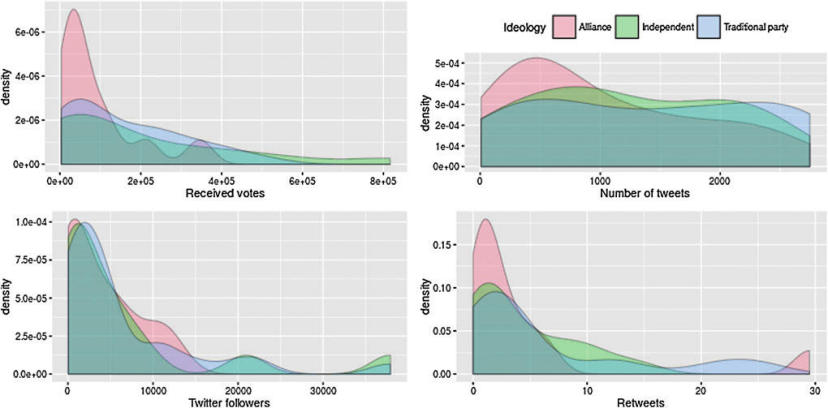
\includegraphics[width=0.55\textwidth]{f1}
\end{figure}
\end{frame}

\begin{frame}{Caso 2: Consumo Ideológico}
Tampoco hubo diferencias estadísticamente significativas en la distribución de la semejanza lingüística entre pares de candidatos según su ideología política; es decir, candidatos representando partidos tradicionales (PP), partidos independientes (II), de alianzas entre partidos (AA), o cualquier otra combinación (F = 1.231; df = 5; p = 0.292).
\begin{figure}
\centering
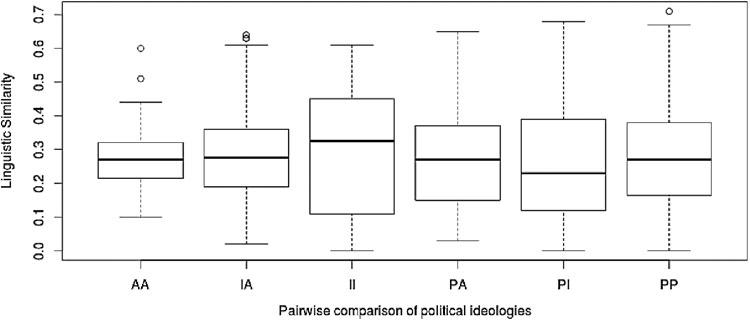
\includegraphics[width=0.7\textwidth]{f2}
\end{figure}
\end{frame}

\begin{frame}{Caso 2: Consumo Ideológico}
La prueba de Shapiro–Wilk sugirió que ni los votos (SW = 0.808; df = 52; p $<$ 0.001) ni los seguidores de Twitter (SW = 0.679; df = 52; p $<$ 0.001), el número de tweets (SW = 0.921; df = 52; p = 0.002), o de retweets (SW = 0.714; df = 52; p $<$ 0.001) mostraban una distribución normal simétrica.
\begin{figure}
\centering
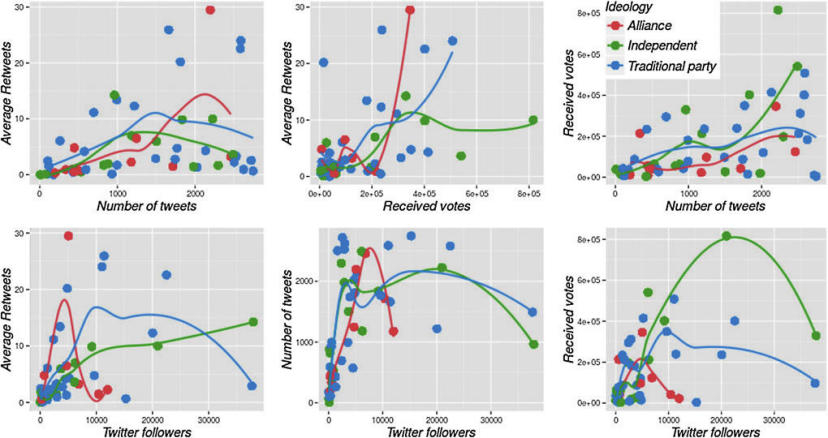
\includegraphics[width=0.55\textwidth]{f3}
\end{figure}
\end{frame}

\begin{frame}{Caso 2: Consumo Ideológico}
Con un modelo de regresión Kernel \cite{Hayfield2008} se evaluó las relaciones multivariadas\\
\vspace{0.5cm}
El modelo mostró resultados altamente ajustados ($R^2$ = \textbf{0.787; p $<$ 0.001}). Los votos se asociaron más fuertemente al número de retweets (Bandwidth = 4.29; p p $<$ 0.01) y de tweets publicados por los candidatos (Bandwidth = 633.06; p = 0.09) que al contenido ideológico de sus mensajes (Bandwidth = 161148.3; p = 0.08) o el número de seguidores en Twitter (Bandwidth = 49,419,488,164; p = 0.37).
\end{frame}

\begin{frame}{Caso 2: Consumo Ideológico}
\begin{itemize}
    \item[1] Se ofreció un análisis diferente sobre el uso de Twitter para propósitos de influencia en campañas electorales.
    \pause
    \vspace{0.5cm}
    \item[2] La aproximación teórica buscaba probar la hipótesis de que la ideología permitía diferenciar claramente el mensaje de los candidatos a gobernaciones, pero los resultados no apoyaron esta idea.
    \pause
    \vspace{0.5cm}
    \item[3] Se demostró un procedimiento empírico fácil de seguir para recolectar grandes tamaños de muestra de datos a partir de Twitter para investigar el consumo ideológico.
\end{itemize}
\end{frame}

\subsection{the Journal of Consumer Psychology}
\begin{frame}
\Large
\centering
¿Y si miramos los tamaños de muestra en los estudios publicados por Journal of Consumer Psychology?
\end{frame}



\begin{frame}{the Journal of Consumer Psychology}
\begin{figure}
\centering
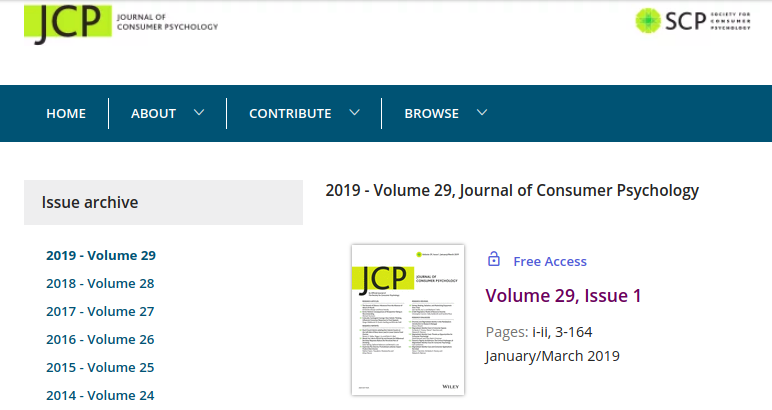
\includegraphics[width=0.9\textwidth]{JCP.png}
\end{figure}
\end{frame}

\begin{frame}{the Journal of Consumer Psychology}
Revisamos un período de 15 meses de publicación (Enero 2018 a Marzo 2019) de trabajos publicados en esa revista para saber cuán frecuente son los trabajos con grandes muestras (i.e., n $\geq$ 10,000).\\
\vspace{0.8cm}
Se descartaron las publicaciones referidas a trabajos teóricos, revisiones de libros, o ensayos, por tratarse de investigaciones que no tienen datos analizables. Encontramos 58 estudios empíricos publicados en el período mencionado. 
\end{frame}

\begin{frame}{the Journal of Consumer Psychology}
En promedio, cualquier paper publicado en JCP reporta un tamaño muestral de 1055 observaciones. El número promedio de experimentos reportados por cada paper está entre 3 y 4 experimentos independientes.
\begin{figure}
\centering
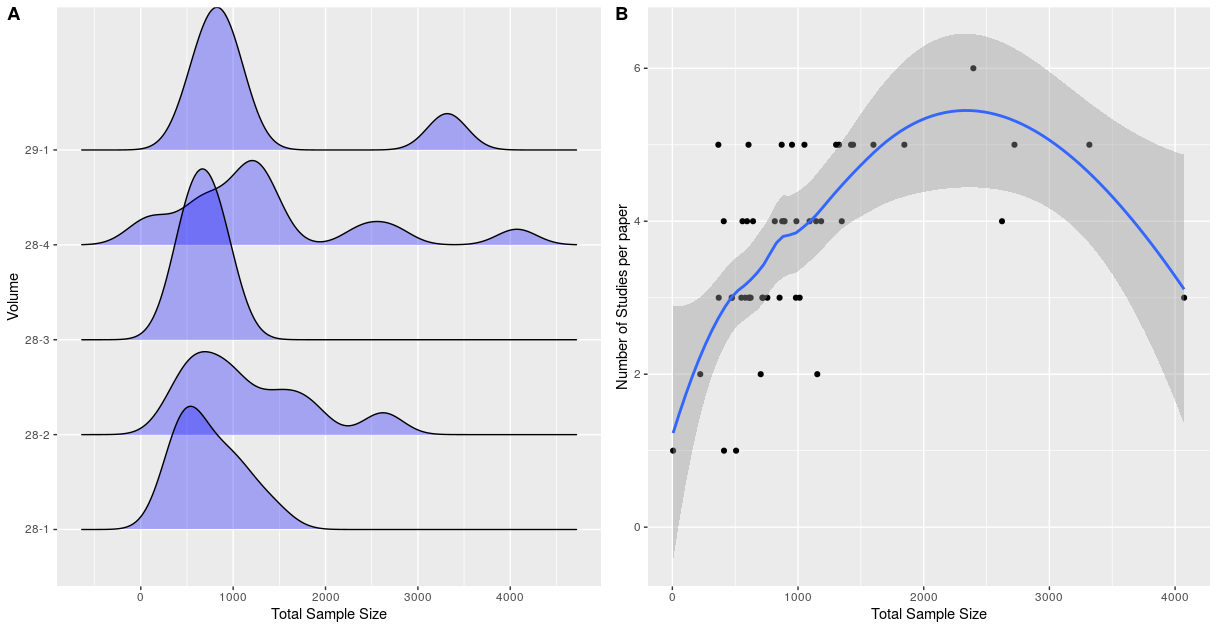
\includegraphics[width=0.9\textwidth]{Figure1.png}
\end{figure}
\end{frame}


\section{Observaciones finales y trabajos próximos}
\begin{frame}{Observaciones finales y trabajos próximos}
\begin{itemize}
    \item[1] En la psicología del consumidor, los tamaños muestrales de $n \geq$10,000 no son comunes.
    \pause
    \vspace{0.5 cm}
    \item[2] Los estudios con n $\geq$ 10,000 se apoyan usualmente en técnicas de recolección de datos no usuales (e.g., cajas registradoras, redes sociales, repositorios).
    \pause
    \vspace{0.5 cm}
    \item[3] ¿Deberíamos enseñar estas técnicas no tradicionales a nuestros estudiantes?
    \pause
    \vspace{0.5 cm}
    \item[4] ¿Son consistentes estos resultados si ampliamos nuestra exploración en el tiempo y exploramos más revistas de investigación del consumidor?

\end{itemize}
\end{frame}

\begin{frame}
\centering
\textbf{¿Preguntas?}
\begin{figure}
\centering
 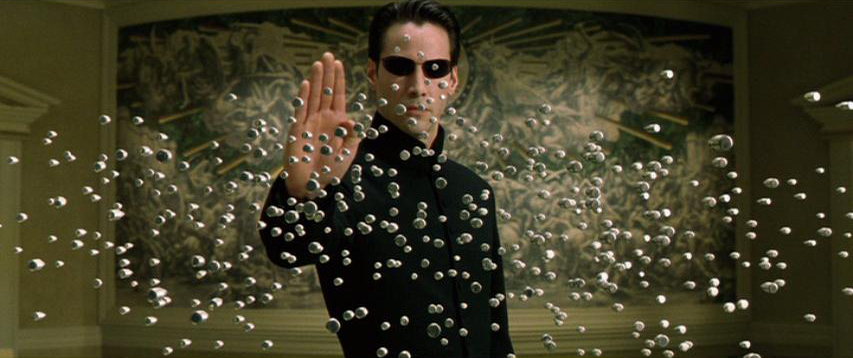
\includegraphics[width=1\textwidth]{Neo}
\end{figure}
\textbf{¡Dispara!}
\end{frame}

\begin{frame}
    \centering
    \Huge
    \textit{¡Gracias!}
\end{frame}


\section*{REFERENCES}
\begin{frame}[allowframebreaks]{References}
\tiny{ 
\bibliographystyle{apacite}
\bibliography{REFS}} 
\end{frame}

\end{document}


